\begin{bibunit}[IEEEtran.bst]

\clearemptydoublepage
\chapter{Problem Formulation and Ontology of Approaches}
\label{chap:1}


\section{The Thermometer Calibration Example}

Journey from an observation problem to a learning problem.
In order to contextualize the work in this thesis, I aim to introduce and explicit the different sources of decision and assumption making when solving an observation problem. This will naturally introduce the concepts used when working with learning-based approaches. Furthermore it will provide a useful perspective for interpreting the research by pointing where learning approaches make different assumptions compared to more traditional approaches.
In order to elucidate the proposed ontology, let's delve into the process of calibrating a thermometer. This example was selected due to its relevance to our study and because it is easier to reason about the underlying physical processes and quantities than in the case of satellite altimetry. As a starting point we can state the problem of calibrating a thermometer as: given an ungraduated thermometer, how can we interpret the level of the liquid as a temperature?

\subsection{Calibrating a thermometer}

The overarching goal of this calibration is to be able to know the temperature at some place by putting the thermometer in a specific location, observe the height of the liquid, and infer the temperature at the point of measurement.

The first step involves accumulating theories and assumptions to construct a model linking the observed level and the actual temperature. For instance, based on our knowledge of fluid dilation in response to temperature, assuming the diameter of the tube is constant with height, we can posit that the level is linearly correlated with the temperature. This model introduces two parameters: the slope and offset of our linear model that need to be ascertained.

The second step involves determining these parameters. For this purpose, we traditionally immerse the thermometer in icing and boiling water to acquire the levels corresponding to 0°C and 100°C. A simple linear system can then be used to solve for the parameters.
This second step rely on data consisting of input-output pairs of the function we're looking for. 

A few notes on this example:
\begin{itemize}
\item The calibration procedure consisted in two steps that respectively rely on conceptual knowledge and data;
\item The two steps are coupled
\item If we loosen the assumption about the tube's constant diameter, we need to incorporate a parameterization of the tube diameter into the model, adding more parameters and necessitating additional data for calibration;
\item If we have a well calibrated thermometer that provides us as many data as we want, we could make very little assumptions and just mark each graduation using data from the calibrated thermometer.
\item By adding the knowledge that the thermometer is in boiling water, our mapping is reduced to a constant function returning 100°C by convention.
  \end{itemize}
% use a report the data points in the graduationswe could limit our assumptions to stationarity (a level that corresponded to a temperature in the past implies the same level corresponds to the same temperature) and smoothness (levels that are close to each other correspond to temperatures that are close to each other), and our temperature estimate could simply be the nearest observation from the data points (which would be a model without parameters);

We now have graduations on our thermometer and can use the level as a proxy for the temperature without further thought!... Although how do we know if our calibrated thermometer is good ? 


\subsection{Evaluation}

Let's define "evaluation" as quantifying quality through metrics.

In our case the most intuitive metric for characterizing our thermometer's quality would be the accuracy of the temperature it gives. However this is by no means obvious, some situation may put greater importance on the speed of the thermometer or the range at which it's functional. 
  Furthermore, in order to properly evaluate our calibrated instrument, we need to test it in conditions corresponding to its intended use, (indeed for a domestic thermometer, testing it it on Mars or 5000 meter underwater would not provide helpful information).

 In order to clarify its intended use, we need to explicit some silent assumptions made on what we would consider a good thermometer.
  For example that it needs to "be accurate to the half of degree", "have response time under 10 minutes", "work between -30°C and 200°C" "work at a reasonnable athmospheric pressure" etc...

Then, using a trustworthy reference like a third-party well-calibrated thermometer, we could compare the measurements of the reference with the one given by our solution.
  An example evaluation procedure could be to confront the measurements of the two instruments at different temperatures such as: in a freezer, in a fridge, at ambiant room temperature and in an oven.

Some remarks about the evaluation:
\begin{itemize}
\item Data is needed for computing metrics
\item The evaluation depend on the metric chosen and the way we compute it.
\item Defining relevant metrics requires intimate knowledge of the intended goal of the instrument.
\item Different metric can produce different rankings, therefore the evaluation is relative to the metric's choice
\item Both the single accuracy in the oven and the mean or standard deviations of the different measured accuracies can be considered as metrics
\item An evaluation can use multiple metrics, therefore no ranking between two methods is guaranteed
\item If the metrics' choice and computation are not suited to the intended use of the instrument, the evaluation will be flawed.
\item If the reference thermometer is biased (not well calibrated) a good metric will not define a thermometer of quality
\item The criterium on the range of the thermometer implies that the thermometer needs to give a temperature even for levels it were not calibrated on (since only finite number of observations were used to calibrate it).
\item If the evaluation only measured the accuracy at the observed temperature 0°C and 100°C, any procedures that fit the observations would get the highest metric even if all other graduations were non-sense.
\end{itemize}

 \subsection{Sources of errors}

Given an evaluation procedure, the errors are the gap to the reference and can be attributed to three sources.
 The model is a source of error if the assumptions made were inacurate. For example if the diameter of the tube is not constant with height the linear correlation between level and temperature is not fallacious and will induce errors when interpreting the level.
 Even with perfect assumptions, the noisy data can introduce errors in the calibration. If we interpreted our 0°C and 100°C in icing and boiling water at the top of a montain with lower athmospheric pressure, we will have calibrated our parameters with erroneous measurements and the subsequent graduation of our thermometer will be inaccurate.
 Finally even with perfect assumption and perfect data, the procedure used to find the solution's parameters can be a source of errors if it fails to find the optimal parameters. For example if we solve for the parameters using a gradient descent method, using a step size too big will prevent finding the exact parameters which will also generate errors in the subsequent measurements.


Once we have an evaluation of our instrument, the next natural step is to aim at reducing the errors. Doing this we're not just thinking about the level-temperature relationship but about the whole method used to determine this relationship. We need to incroporate in our reasoning the how the calibration method (assumptions, data, optimization) relates to the errors we measure. We can state this as a higher level problem: "How to find the best thermometer calibration procedure?"

\subsection{Finding the best thermometer calibration procedure}
In this section, we propose a parallel between the two problems of "knowing the temperature when looking at the thermometer" and  "knowing the calibration procedure". we respectively call first order and second order what refers to the former and latter.

  The second order objective is to find a function that takes in a set of level-temperature observations, and returns the level to temperature mapping (the first order solution)

In order to find such a procedure, we can apply the same two steps as before.

  First, how to model the link from the input observations and the output mapping. This would include (first order) assumptions about the relationship between level and temperature as well as assumptions about the type of errors in the observations and the optimization procedure. These different assumptions are compiled into a set of candidate calibration procedures characterized by some configuration (the second order parameters).

  The second step consists then in determining the optimal configuration among the different candidates.
  When considering the first order problem, the data used to determine the parameter were levels with corresponding temperature. These data are  the inputs and outputs of the function we are trying to determine.
  If we reason about the inputs and outputs of our calibration procedure, the inputs consists in a set of level-temperature pairs  and the output are calibrated thermometer.
  Indeed 
  
  In order to do so, we need data points as well as an evaluation procedure.


A few notes on this example:
\begin{itemize}
\item The same two steps applied for the first and second order problem: defining candidates using theory and finding the optimal solution using data
\item A second order solution is a function that takes as inputs first order data and outputs first order solution
\item Second order parameters can be discrete choices like different first order assumptions 'considering the diameter is constant or not'
\item Second order parameters can be discrete choices between two different optimization procedure
\item Second order parameters can be constants in the level-temperature mappings
\item Second order parameters can be parameters of an optimization procedure like step size
\item The first order assumptions are about the physics of the system 
\item The second order assumptions includes considerations about the methods through data (errors) and optimization
\end{itemize}

We now have a great calibration procedure!... Or do we?  Wait what is a "great" calibration procedure?

\subsection{Evaluation of a calibration procedure}

A first question we need to ask to evaluate the procedure in itsefl is: what would be the desired domain (i.e. range) of a calibration procedure ? Or put differentely, on what calibration problems do we intend to use it.
We therefore need to explicit what kind of thermometer we want the calibration procedure to be applied to, and what observations we expect to have.
In our example, I implicitely wanted the calibration procedure to work on any standard thermometer, having at least two level-temperature observations without noise.

Now we need to determine a metric and an evaluation procedure.

Having determined a satisfying metric for evaluating a thermometer, a natural metric for the procedure is to compute the calibration metric on results of the procedure
The evaluation procedure can then be to use a few different thermometers a verify that the caliration works well on them.


A few remarks here:
\begin{itemize}
\item other metrics can relate to second order aspects of the problem, for example the robustness to noise or the computational complexity.
\item Different calibration tasks need not be on multiple thermometers, but could the same thermometer with different observation data points
\item if we tuned our procedure and computed our metric on a single thermometer, the metric would not informed us if the calibration worked on different thermometer.
\end{itemize}


Using this evaluation procedure, we could quantify the second order errors that could be classified in the same categories.
The model errors now includes the repercussions of wrong assumptions and parameterizations of errors in the data and optimization dynamics.
Data errors would for example be due an inaccurate reference thermometer used tune the second order parameters.
And optimization errors denote the gap between the solution found compared to the best possible candidate when evaluated on second step's data.


\subsection{Introducing space}
  As mentioned in the notes ultimate objective (zero order) of the calibration is to know the temperature at a single place and time given by the location of the thermometer. 
  This is a particular case  -- related to the calibration task  -- of the classes of problem we're interested in.
  The more generic class of problems would be knowing the temperature field over a spatio-temporal domain.

We could then update the associated hierarchy of problems as:
  - Zero order: Know the temperature given a location and a time within a spatio-temporal frame, 
  - First order: Find the field of temperature given observations of thermometers (potentially at different places and times)
  - Second order: Determine a procedure that can map a set of observation to the temperature field

And the conceptual blocks introduce above apply in a similar manner.


  As mentioned in the notes ultimate objective (zero order) of the calibration is to know the temperature at a single place and time given by the location of the thermometer. 
  This is a particular case  -- related to the calibration task  -- of the generic classes of problem we're interested in.
  The more associated generic class of problems would be knowing the temperature field over a spatio-temporal domain.

We could then update the associated hierarchy of problems as:
  - Zero order: Know the temperature given a location and a time within a spatio-temporal frame, 
  - First order: Find the field of temperature given observations of thermometer levels (potentially at different places and times)
  - Second order: Determine a procedure that can map a set of observation to the temperature field

And the conceptual blocks introduce above apply in a similar manner.


\subsection{In a nutshell}

A necessary step before developing a solution to a problem is to be able to evaluate it, this requires informed knowledge and assumptions on the intended use of the solution as well as a choice of metric computation and the associated data.

Then to actually develop the solution, three components are needed: a model of the relationship between input and output of the solution as well algorithm to chose the model configuration given some data.


To solve the calibration problem we need to come up with a calibration procedure that will take level-temperature observations to produce the calibrated thermometer.

To evaluate the calibration procedure we evaluate the calibrated thermometers over a range of representative tasks.
To evaluate a calibrated thermometer, we compare the temperatures given by the thermometer over a range of representative situations.

To develop the calibration procedure we need three components:
The data: an ensemble of calibration task that we can evaluate (of calibrated thermometers)
The algorithm that choses the best calibration procedures 
The model that is the set of candidates calibration procedures that differ by one or more component:
  The model which is the set of candidate of level-temperature mapping
  The algorithm that choses the best mapping given some level-temperature observations







Solving an observation problem can be structured in two levels:
- Finding the best estimate of the temperature when looking at a thermometer
- Finding the best way to convert observations 
- Linking the observation to the quantity of interest

\subsection{Domain experts versus deep learning approaches}
  We group what we describe above in the domain experts category of methods, with a tendency 




\section{Generic formulation}

  The zero order objective of the class of problem we're interested in is to find a function $f_0=\hat{u}$  that approximates a quantity of interest $u(t, x)$ on a domain $\Gamma_u$ with values in $\mathbb{R}^d_u$. 
  In geoscience we can generally consider $\Gamma$ to be spatio-temporal, and define the spatial and temporal domains  as {\Omega = {x, (t,x) \in \Gamma} and {\Tau = {t, (t,x) \in \Gamma}

   $u$ is defined 
  conditioned on a set of observations $\cal{D}_0$.

  The first order objective is therefore to formulates $f_1$ that outputs $f_0$ from  a set of observations $\cal{D}_0$
  with $\cal{D}_0 = \{(p_1, y(p_1)), ..., (p_{N_0}, y(p_{N_0})) \}$ with  $p_i \in \Gamma_y$ and $y: \Gamma_y \to \mathbb{R}^d_y$.

  The second order objective is therefore to formulates $f_2$ that outputs $f_1$ from a dataset $\cal{D}_1$ .
  with $\cal{D}_1 = \{(cal{D}_0^1, Y^1),... (cal{D}_0^{N_1}, Y^2) \}$ with  $cal{D}_0^{i}$ different sets of observations and $Y^i$ additional data that can be used to evaluate first order solutions.

  We note $\cal{F}_1$  the set of candidates $f_1$ and $\theta_1 \in \mathbb{R}^p_1$ the parameters of $f_1$
  We note $\cal{F}_2$  the set of candidates $f_2$ and $\theta_2 \in \mathbb{R}^p_2$ the parameters of $f_2$



% We could then state that a second order metric is can be composed of first order metrics.
%
% Some 
%
% The domain 
%
% We can then 
%
% We can use analog steps as for the evaluation of the calibrated thermometer to reason about the assessment of the quality of the calibration procedure.
%
% 1) What assumptions did we make about what is a good calibration procedure ?
% 2) What metric would be a good way a quantifying them ?
% 3) How can we compute this metric in a representative way ?
%
%
% A first idea to assess if our calibration procedure is good, would be to evaluate our thermometer once calibrated with it.
% However we would then be faced with a dilemna, 
% The issue encountered is that if we use the same evaluation procedure we 
% The most straightforward idea for a good k
%
%  Indeed the best possible calibration procedure will certainly produce a weakly calibrated thermometer if the input observations associate random levels with random temperatures.
%
%
%
% Those are the three sources of error from our calibration procedure, however note that in the absence of perfect reference we cannot directly quantify them.
%  Then as is often the case, some proxy is used as another source of error is even trickier and comes from the gap betkno In the absence of such reference we could 
% A reference 
% We would like to clarify that the evaluation procedure needs to be done on data that were not used 
%  Evaluating a second order solution on a data point uis
% Evaluating a second order solution only makes sense if the evalua
% We first want to point out the importance of the scope of evaluation, the second order problem only makes sense
%
% \subsection{Introducing time}
% The response time of the thermometer is the duration before the temperature indicated by the level reflects the temperature of the location it's in. This is related to the fact that the level is actually related to the temperature of the liquid which will take some time to adjusts to the location temperature.
% One could aim at using the thermometer to estimate the instantaneous temperature.
% However, in order to do so multiple recent observations at the same location  would be needed to take into account the dynamics.
% The mapping between recent observations and instantaneous temperature would include a parameterization of the diffusion process.
% The evaluation should also be consciensiously chosen to measure the dynamical aspects.
%
% Note that this could be treated as an end to calibration problem if we consider the levels as the thermometer as inputs, or as a separate problemif we consider the thermometer already graduated. This would impact the different hypothesis made.
%
%
%
%
% %###################
%
%
% \begin{itemize}
%   \item The optimization procedure also relies on some assumptions and parameters
%   \item We can then think of the tuning of hyper-parameters as an a higher order problem
%   \item The solution of this problem takes in a set of data points and produces a mapping between levels and temperatures.
%   \item Such solution could be applied to a range of different thermometer given that the set of available data points meets the requirements
%   \item The accuracy of a calibrated thermometer would depend on the validity of the assumptions made
% \end{itemize}
%
% \section{Problem Formulation Bis}
% \label{sec:chap1_problem_formbis}
%
%   The end objective (zero order) of the class of problem we're interested in is to find a function $f_0=\hat{u}$  that approximates a quantity of interest $u(t, x)$ conditioned on a set of observations $\cal{D}_0$.
%    $u$ is defined on a domain $\Gamma_u$ with values in $\mathbb{R}^d_u$.
%   In geoscience we can generally consider $\Gamma$ to be spatio-temporal, and define the spatial and temporal domains  as {\Omega = {x, (t,x) \in \Gamma} and {\Tau = {t, (t,x) \in \Gamma}
%   A set of observations is in the form $\cal{D}_0 = \{(p_0, y(p_0)), ..., (p_{N_y}, y(p_{N_y})) \}$ with  $p_i \in \Gamma_y$ and $y(p_i) \in \mathbb{R}^d_y$.
%
%
%   Therefore, $f_0 \in \cal{F}_0 = { h \to \alpha h + \beta , (\alpha, \beta) \in |R^2 }$.
%
%   More generally, $f_0 \in \cal{F}_0 = \{ f: y; z \to f(y; z), z \in |R^{N_0} \}$ with f the modelisation of the first order problem parameterizes by $z$.
%
%
%   Solving for $f_0$ consists in two steps: 
%   Defining $\cal{F}_0$  the set of candidate $f_0$ and $\theta_0 \in \mathbb{R}^p_0$ the parameters of $f_0$
%   Defining the procedure $f_1$ that outputs $f_0$ from $\cal{D}_0$
%
%
%   The first order objective is therefore to formulates $f_1$ that outputs $f_0$ from $\cal{D}_0$
%   We note $\cal{F}_1$  the set of candidate $f_1$ and $\theta_1 \in \mathbb{R}^p_1$ the parameters of $f_1$
%
%   We can similarly introduce a second order objective which is to find $f_2$ that outputs $f_1$ from  $\cal{D}_1$ which groups multiple observation sets 
%   We note $\cal{F}_1$  the set of candidate $f_1$ and $\theta_1 \in \mathbb{R}^p_1$ the parameters of $f_1$
%
% All along this section we will illustrate our ontology of problems and methods using an example of thermometer calibration. We chose this use case due to its relevance to our work given that it's about sensor calibration and because the underlying physical processes are much simpler that the ones involved in the earth system wich makes for a comprehensive and useful usecase.
%
% In the case of our thermometer the quantity of interest is the temperature  $T$ which is a scalar field and $\Omega_u$ is the thermometer location  $x_t$ at time $t_t$. 
%   We want to estimate it given a single observation of the level of the thermometer $h_t$ at the same point: $\cal{D}_0 = \{((x_t, t_t), h_t$.
%
%   In the case of our thermometer, $f_1: \{(t_t, x_t, h_t)\} -> \{f_0(t_t, x_t)\}$ can be reduced  to finding the relationship between the level $h_t$ and the temperature $T_t$ of the thermometer.
%
%
%   In order to solve the first order problem, the first step involves compiling our theoretical knowledge and making assumption to come up with a model. For example, given our understanding of fluid dilation in response to temperature, under the assumption that the diameter of the tube is constant with height, can assume that level is linearly correlated with the temperature. Therefore, $f_1 \in \cal{F}_1 = { h \to \alpha h + \beta , (\alpha, \beta)=\theta_1 \in |R^2 }$.
%     A second necessary step is to determine the values of $\alpha$ and $\beta$. To this end we require a set of data points $\cal{D}_1 = \{\cal{D}_0^1=(h^1, T^1), ..., \cal{D}_0^{N_1}=(h^{N_1}, T^{N_1})\}$ to calibrate our model, traditionally obtained by placing the thermometer in icy and boiling water to get the levels corresponding to 0°C and 100°C. We can then solve for the parameters with a simple linear system.
%
%
%
%
%   The second order objective is then to formulates $f_2$ that outputs $f_1$ from  $\cal{D}_1$
%
%
%   We can now formulate the second order problem associated with 
%   The 
%    To solve this 
%   The end objective of the class of problem we're interested in is to find a function $f_0$  that approximates a quantity of interest $u(t, x)$ on a domain $\Gamma_u$ with values in $\mathbb{R}^d_u$.
%   In order to estimate find $f_0$, we have observation data $\cal{D}_0 = \{(p_0, y(p_0)), ..., (p_{N_y}, y(p_{N_y})) \}$ with  $p_i \in \Gamma_y$ and $y(p_i) \in \mathbb{R}^d_y$.
%   In geoscience we can generally consider $\Gamma$ to be spatio-temporal, and define the spatial and temporal domains  as {\Omega = {x, (t,x) \in \Gamma} and {\Tau = {t, (t,x) \in \Gamma}
%
%
% \section{Problem Formulation}
% \label{sec:chap1_problem_form}
%
%
%
% The broadest formulation the problems we're interested in is finding a function $f$ which maps the available inputs $y$ to the desired outputs $u$.
%
%
%
%
%
% All along this section we will illustrate our ontology of problems and methods using an example of thermometer calibration. We chose this use case due to its relevance to our work given that it's about sensor calibration and because the underlying physical processes are much simpler that the ones involved in the earth system.
%
% This formulation encompasses different order of problem that we detail below.
%
% \subsection{First order: Calibrating the thermometer}
%   \label{ssec:firstorder}
% The first order of problem would be to find the mapping $f_0$ between a given level $h$ of the thermometer and the associated temperature $T$ of the liquid within.
%
% A first step would involve compiling our theoretical knowledge and making assumption to come up with a model. For example, given our understanding of fluid dilation in response to temperature, under the assumption that the diameter of the tube is constant with height, if we don't know the volume of liquid and the dilation rate we can model an affine  that the level is linearly correlated with the temperature. Therefore, $f_0 \in \cal{F}_0 = { h \to \alpha h + \beta , (\alpha, \beta) \in |R^2 }$.
%
%   More generally, $f_0 \in \cal{F}_0 = \{ f: y; z \to f(y; z), z \in |R^{N_0} \}$ with f the modelisation of the first order problem parameterizes by $z$.
%
%   A second necessary step is to determine the values of $\alpha$ and $\beta$. To this end we require a set of data points $\cal{D}_0 = \{(h^1, T^1), ..., (h^{d_0}, T^{d_0})\}$ to calibrate our model, traditionally obtained by placing the thermometer in icy and boiling water to get the levels corresponding to 0°C and 100°C. We can then solve for the parameters with a simple linear system.
%
%
%   The first and second step are coupled. Indeed, the more parameters $f_0$ depends on, the more data points will be needed in $\cal{D}_0$
%   For example if some assumptions are considered too restrictive like "the diameter of the thermometer is constant with height", they can be relaxed.
%   However this expands the class of functions $F_0$, by requiring the incorporation of a model of the diameter in function of height, which will introduce new parameters. Let's assume that the diameter is linear per part for every $K$mm section, and the corresponding parameters to find would be the $N_k$ value of the diameter every $K$mm: $(d_1, ... d_{N_k}) \in |R^{N_k}$ 
%
%   In this new formulation, note that chosing $d_i$ values determi
%   In order to find adequate $d_i$ values, more data points would be needed in $\cal{D}_0$
%
% \subsection{Second order: Finding a thermometer calibration procedure}
%   The resolution of a first order problem can be stated as the following: How to find the mapping $f_1$ between a set of data points $\cal{D}_0$ and $f_0$.
%   We refer to this formulation as a second order problem.
%
%   The second order solution $f_1$, is a procedure that outputs the best first order solution given a set of data points $\cal{D}_0$
%   This procedure is an algorithm chosen in regard of some assumptions on the level of noise in the input $\cal{D}_0$ and the landscape of the search space $F_0$. These assumptions define the classes of functions $\cal{F}_1 = \{f: \cal{D}_0; \theta \to f_0, \theta \in |R^{N_1}\}$ conditionned on $\theta$ which are the constant parameters across first order instances.
%   In the above example $f_1$ could be the resolution of a simple linear system without any parameters, but could also be a gradient descent procedure relying on a definition of an objective function and with parameters such as the step size. 
%   More generally, when focusing on iterative optimization procedure such as gradient descent based algorithms, the parameters \theta can be characterize initialization schemes, the step computation or regularization parameters that reduce the search space $F_0$.
%
%
%   % Note that regularization can be loosely defined as assumptions used to reduce the search space $\cal{F}_0$ across all tasks such that $f_0 \in \cal{F}_0 = \{ f: y; z \to f(y; z), z \in \cal{Z}(\theta) \subset |R^{N_0} \}$.
%   % An example of regularization assumption could be a smoothness a priori on the diameter of the thermometer conditionned on a parameter $\lambda$ such that the parameters $(d_1, ... d_{N_k}) \in |R^{N_k}$ are constrained by  $\forall i \in [|1, N_k-1|], d_i - d_{i+1} < \lambda$ effectively reducing the search space.
%
%   The parameters $\theta$ are then tuned using a dataset $\cal{D}_1 = \{\cal{D}_0^1, ..., \cal{D}_0^{d_1}\}$ comprised of multiple instances of first order problems.
%
%  For example one can use the different examples in  $\cal{D}_1$ 
%
% %   We when modeling The function $f_1$ also depends on parameters that are 
% %   Additionally, for second order problems, the solution $f_1$ performs the search for the parameters of $f_0$ i.e. an optimization procedure. This procedure also depends on assumptions such as the level of noise in the input $\cal{D}_0$, and the landscape of the search space $F_0$. This will define parameters to find for $f_1$. Such parameters are tuned using a dataset $\cal{D}_1 = \{\cal{D}_0^1, ..., \cal{D}_0^{d_1}\}$ comprised of multiple first order problems.
% %
% %
% % Finally some parameters of the modelisation of first order problem can be unknown but common across problems and therefore are parameters of 
%
%
% \subsection{Second order ++: Finding a generic procedure to solve a class of problem}
%
% In the above second order problem, note that the class of function $F_0$ considered needs now to apply to every thermometers we want to calibrate using $f_1$.
%
%   This can motivate the elaboration of more generic modelisation $f_0$ with higher dimensional $cal{\F}_0$.
%   However this requires more data.
%   The two sources of data $\cal{D}_0$ and $\cal{D}_1$ are complimentary to this end.
%   More data in $\cal{D}_1$ allow for more tuning more parameters generic across and therefore reducing the search space of $cal{\F}_0$ during the second order resolution.
%   whereas a larger $\cal{D}_0$ can be used to search higher dimensional $cal{\F}_0$ during the first order resolution.
%
%   In the thermometer example above assuming the determination of the diameter every $K$mm requires too much datapoints compare to what we expect to have in $\cal{D}_0$, but that we have a many examples of thermometers in $\cal{D}_1$.
%   We can learn the distribution 
%   We could then introduce regularization parameters to be fitted across different first order instances and that would couple the $d_i$ together such as reducing the search space of $F_0$.
%   For example coupling the 
%   degrees of freedom that can be solved for each $\cal{D}_0$
%
%
% In the previous example, we saw an example of broadening the space of possible first order solution by relaxing some assumptions and then searching this larger space relying on more data.
% Going even further we could aim at finding a generic approach for finding calibration operator of differnt kind of sensors or even generic 
%
%
%
%
%   The model of the thermometer made for the first order problem needs to be questioned and 
%   When solving a second order problem, the assumptions made to 
%   $f_1$ then incorporate the search for $f_0$'s parameters.
%
%
%
% Given a non graduated thermometer we want to find 
%
%
% In geoscience, $u$ and $y$ can generally be defined as $D_u$ and $D_y$ dimensional vector fields defined on spatio-temporal domains $\Omega_u$ and $\Omega_y$. Here, we consider scalar fields and discrete fields as particular cases of this generic formulation. The different problems can be characterized by the types of quantities $u$ and $y$ and the spatio-temporal domains $\Omega_u$ and $\Omega_y$ on which they are defined. Figure \ref{fig:planet_drawings} illustrates how our two use cases of sensor calibration and SSH mapping easily fit into such formulation. Additionally, Figure \ref{fig:task_ontology} shows how tasks such as calibration, mapping, and forecasting can differ through the domain of definition of $u$ and $y$.
%
% \begin{figure}[htbp]
% \begin{center}
% 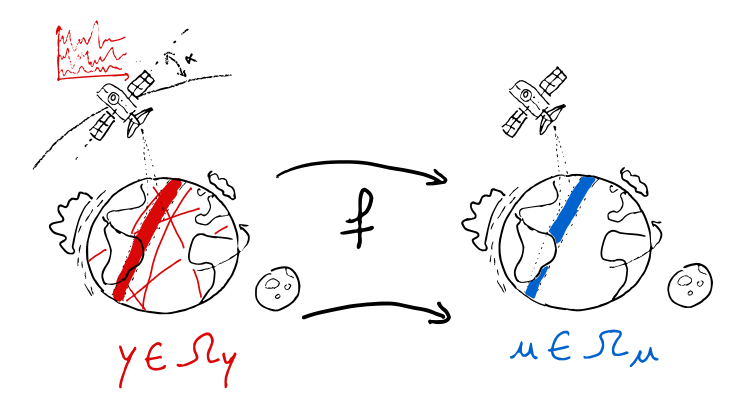
\includegraphics[width=0.8\linewidth]{Chapitre1/Ch1-Figures/Cal_drawing.png} 
% 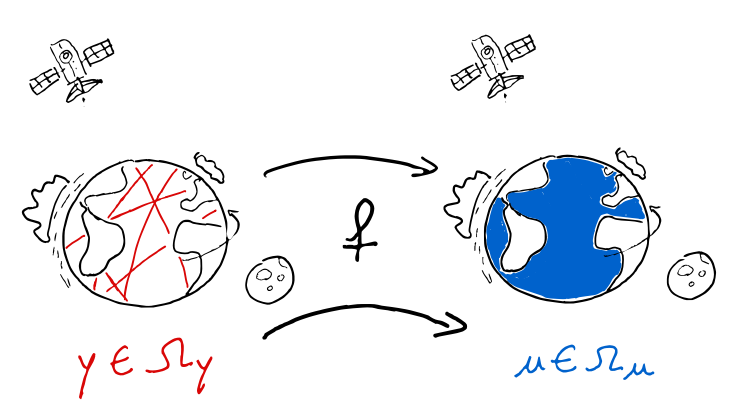
\includegraphics[width=0.8\linewidth]{Chapitre1/Ch1-Figures/Mapping_drawing.png} 
% \end{center}
% \caption[Swot calibration and altimetry mapping problem illustration]
% {\footnotesize The calibration problem (top row) consists in finding the mapping $f$ that estimates the observed SSH $u$ from the SWOT satellite given the actual noisy measurement and ancillary calibrated measures ($y$).
% The mapping task (bottom row) consist in finding an operator $f$ that maps partial measurements of the SSH $y$ to a map of SSH $u$}
% \label{fig:planet_drawings}
% \end{figure}
%
%
% % \begin{figure}[htbp]
% % \begin{center}
% % \begin{tabular}[c]
% % 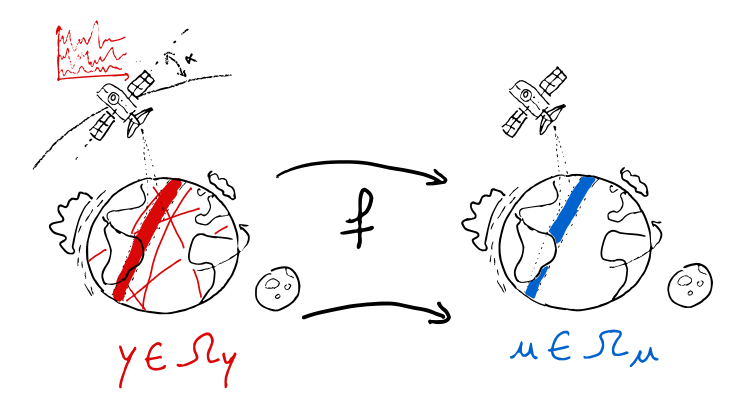
\includegraphics[width=0.8\linewidth]{Chapitre1/Ch1-Figures/Cal_drawing.png} \\
% % 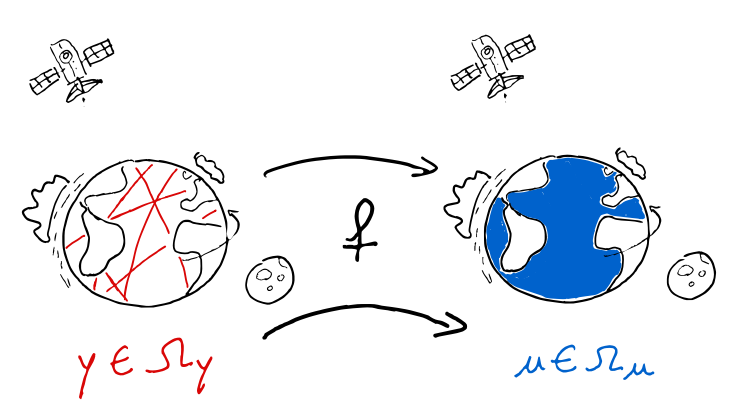
\includegraphics[width=0.8\linewidth]{Chapitre1/Ch1-Figures/Mapping_drawing.png} \\
% % \end{tabular}
% % \end{center}
% % \caption[Swot calibration and altimetry mapping problem illustration]
% % {\footnotesize The calibration problem (top row) consists in finding the mapping $f$ that estimates the observed SSH $u$ from the SWOT satellite given the actual noisy measurement and ancillary calibrated measures ($y$).
% % The mapping task (bottom row) consist in finding an operator $f$ that maps partial measurements of the SSH $y$ to a map of SSH $u$}
% % \label{fig:planet_drawings}
% % \end{figure}
%
% \begin{figure}[htbp]
% \begin{center}
% 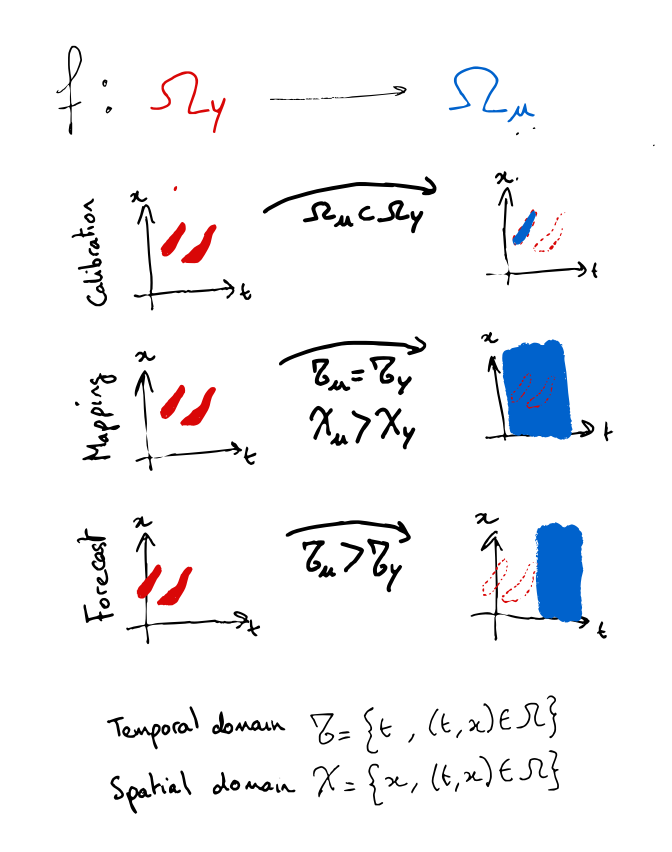
\includegraphics[width=0.8\linewidth]{Chapitre1/Ch1-Figures/Task_ontology.png}
% \end{center}
% \caption[Task characterization through the domains $\Omega_u$ and $\Omega_y$ of $u$ and $y$]
% {\footnotesize Using the perspective provided by the problem definition, we can easily categorize earth observation problems.
% The calibration consist of estimating the field $u$ on a subset of the observation domain, the mapping consist in estimating $u$ on the same temporal domain but extending the spatial domain.
% And finally forecast can considered as wanting to estimate a quantity on an unobserved future domain.}
% \label{fig:task_ontology}
% \end{figure}
%
% \section{Method Ontology}
% We aim to characterize and organize the various methods used to tackle the class of problem introduced in \ref{sec:chap1_problem_form}. We propose that all methods can be decomposed into the following two steps:
% \begin{itemize}
% \item Step 1: Define the set $\cal{F}$ of possible $f$ using theoretical knowledge and making assumptions about the problem (conceptual models)
% \item Step 2: Search $\cal{F}$ for an optimal $f$ using factual knowledge (data) and making assumptions about the data
% % \item The first and second steps respectively rely on conceptual knowledge and available data;
% % \item If the data had included the volume of the liquid, the tube's diameter, and the dilation rate of the liquid, we might have needed theoretical knowledge about the volume of a tube to construct a relationship between the level and the temperature;
% % \item If only the diameter were unknown in a similar situation, a single data point would have been sufficient to calibrate the model;
% \end{itemize}
%
%   To illustrate our point let's consider the simple problem of thermometer calibration.
%
%
%
%
%
% To illustrate our point, consider a simple example of building a thermometer by placing a liquid in a tube and wanting to interpret the level of the liquid as a temperature. According to our previous notations, $y$ is the level of the liquid and $u$ is the temperature of the liquid inside, and we seek to find the mapping $f$ between the two.
%
% Step 1 involves compiling our theoretical knowledge on the problem to define the class of function. Given our understanding of fluid dilation in response to temperature, under the assumption that the diameter of the tube is constant with height, we can state that the level is linearly correlated with the temperature. Therefore, $f$ will be part of $\cal{F} = { y: \alpha y + \beta , (\alpha, \beta) \in |R^2 }$.
%
% In Step 2, to find $\alpha$ and $\beta$, we require two data points to calibrate our model, traditionally obtained by placing the thermometer in icy and boiling water at 1 bar of pressure to get the levels corresponding to 0°C and 100°C. This method relies on strong theoretical foundations and assumptions to reduce the dimensionality of the search space $\cal{F}$, thus facilitating the parameter search with relatively few data points.
%
% However, if we clearly see that the diameter of our thermometer is not constant, the model needs to incorporate that the evolution of the temperature depends on the diameter at each height. This expands the class of functions, necessitating the incorporation of a model of the evolution of the diameter in function of the height, which will introduce new parameters. We could assume that the diameter is linear for every 5mm section, and the corresponding parameters to search would be the value of the diameter every 5mm.
%
% To estimate these new parameters, we need more data which could be direct measures of the diameter or measures of temperature every 5mm. We could directly model $f$ as linear per part, thereby reducing the number of parameters to estimate (no more $\alpha$ and $\beta$). If we have measurements of the temperature, this also alleviates the need to explicitly model the relationship between diameter and temperature.
%
%
%
%
%
%
% % Tasks
% % Simple exemple
% % Calibration and mapping example
%
% % Tasks of interests can be summed up as finding f
% % Finding f takes two steps: defining the set of possible fs, searching the set for the best f
% % Formulating the sets of F requires theoritical knowledge
% % Searching the sets of F requires data
%
% % From theory to sets of 
% %   inverse problems state x
% %   data assimilation: dynamical model
% %   spatio temporal correlation: Covariance model
% %   deep learning
% %   locality: convolution
% %   temporal dependence RNN LSTM
%
%
% Lorem ipsum dolor sit amet, consectetuer adipiscing elit. Maecenas fermentum, elit non lobortis cursus, orci velit suscipit est, id mollis turpis mi eget orci.
%
% \section{Première section du chapitre}
%
% Lorem ipsum dolor sit amet, consectetuer adipiscing elit. Maecenas fermentum, elit non lobortis cursus, orci velit suscipit est, id mollis turpis mi eget orci.
%
% \subsection{Première sous-section}
%
% Lorem ipsum dolor sit amet, consectetuer adipiscing elit. Maecenas fermentum, elit non lobortis cursus, orci velit suscipit est, id mollis turpis mi eget orci.
%
% Voir figure \ref{fig:mafigure2}.
%
%
% \begin{figure}[htbp]
%    \begin{center}
%       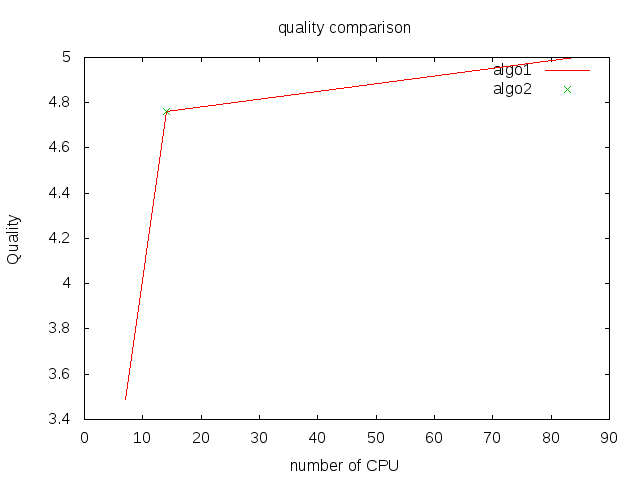
\includegraphics[width=0.8\linewidth]{Chapitre1/Ch1-Figures/comparison.png}
%    \end{center}
%    \caption[titre court pour la liste des figures]
%    {\footnotesize Titre plus long avec des explications.}
%    \label{fig:mafigure2}
% \end{figure}
%
% \subsection{Deuxième sous-section}
%
% The calibration procedure described above followed an intuitive flow of framing the problem using assumptions on the physics and solving it using data.
% The calibration procedure described above followed an intuitive flow of framing the problem using assumptions on the physics and solving it using data.
%
% The above section detailed how to find a function that maps an observation of the level of the thermometer to the temperature.
% We saw how this function is the result of an procedure that uses some assumptions about the problem and takes as input a set of data points.
%
% We propose here a parallel between the calibration problem as stated above and the optimization problem of infering optimal parameters from data-points.
%
% The first step 
%
% Lorem ipsum dolor sit amet, consectetuer adipiscing elit. Maecenas fermentum, elit non lobortis cursus, orci velit suscipit est, id mollis turpis mi eget orci.
%
% \section{Conclusion du premier chapitre}
%
% Lorem ipsum dolor sit amet, consectetuer adipiscing elit. Maecenas fermentum, elit non lobortis cursus, orci velit suscipit est, id mollis turpis mi eget orci.
%
% In this manuscript I'd like to cite \cite{remo3,remo4}.

\addcontentsline{toc}{section}{Bibliography}
\putbib[./Chapitre1/Ch1-Biblio.bib]
\end{bibunit}
